\documentclass{standalone}
\usepackage{tikz}
\usetikzlibrary{patterns, positioning}
\usepackage[sfdefault]{ClearSans} %% option 'sfdefault' activates Clear Sans as the default text font
\usepackage[T1]{fontenc}

\begin{document}
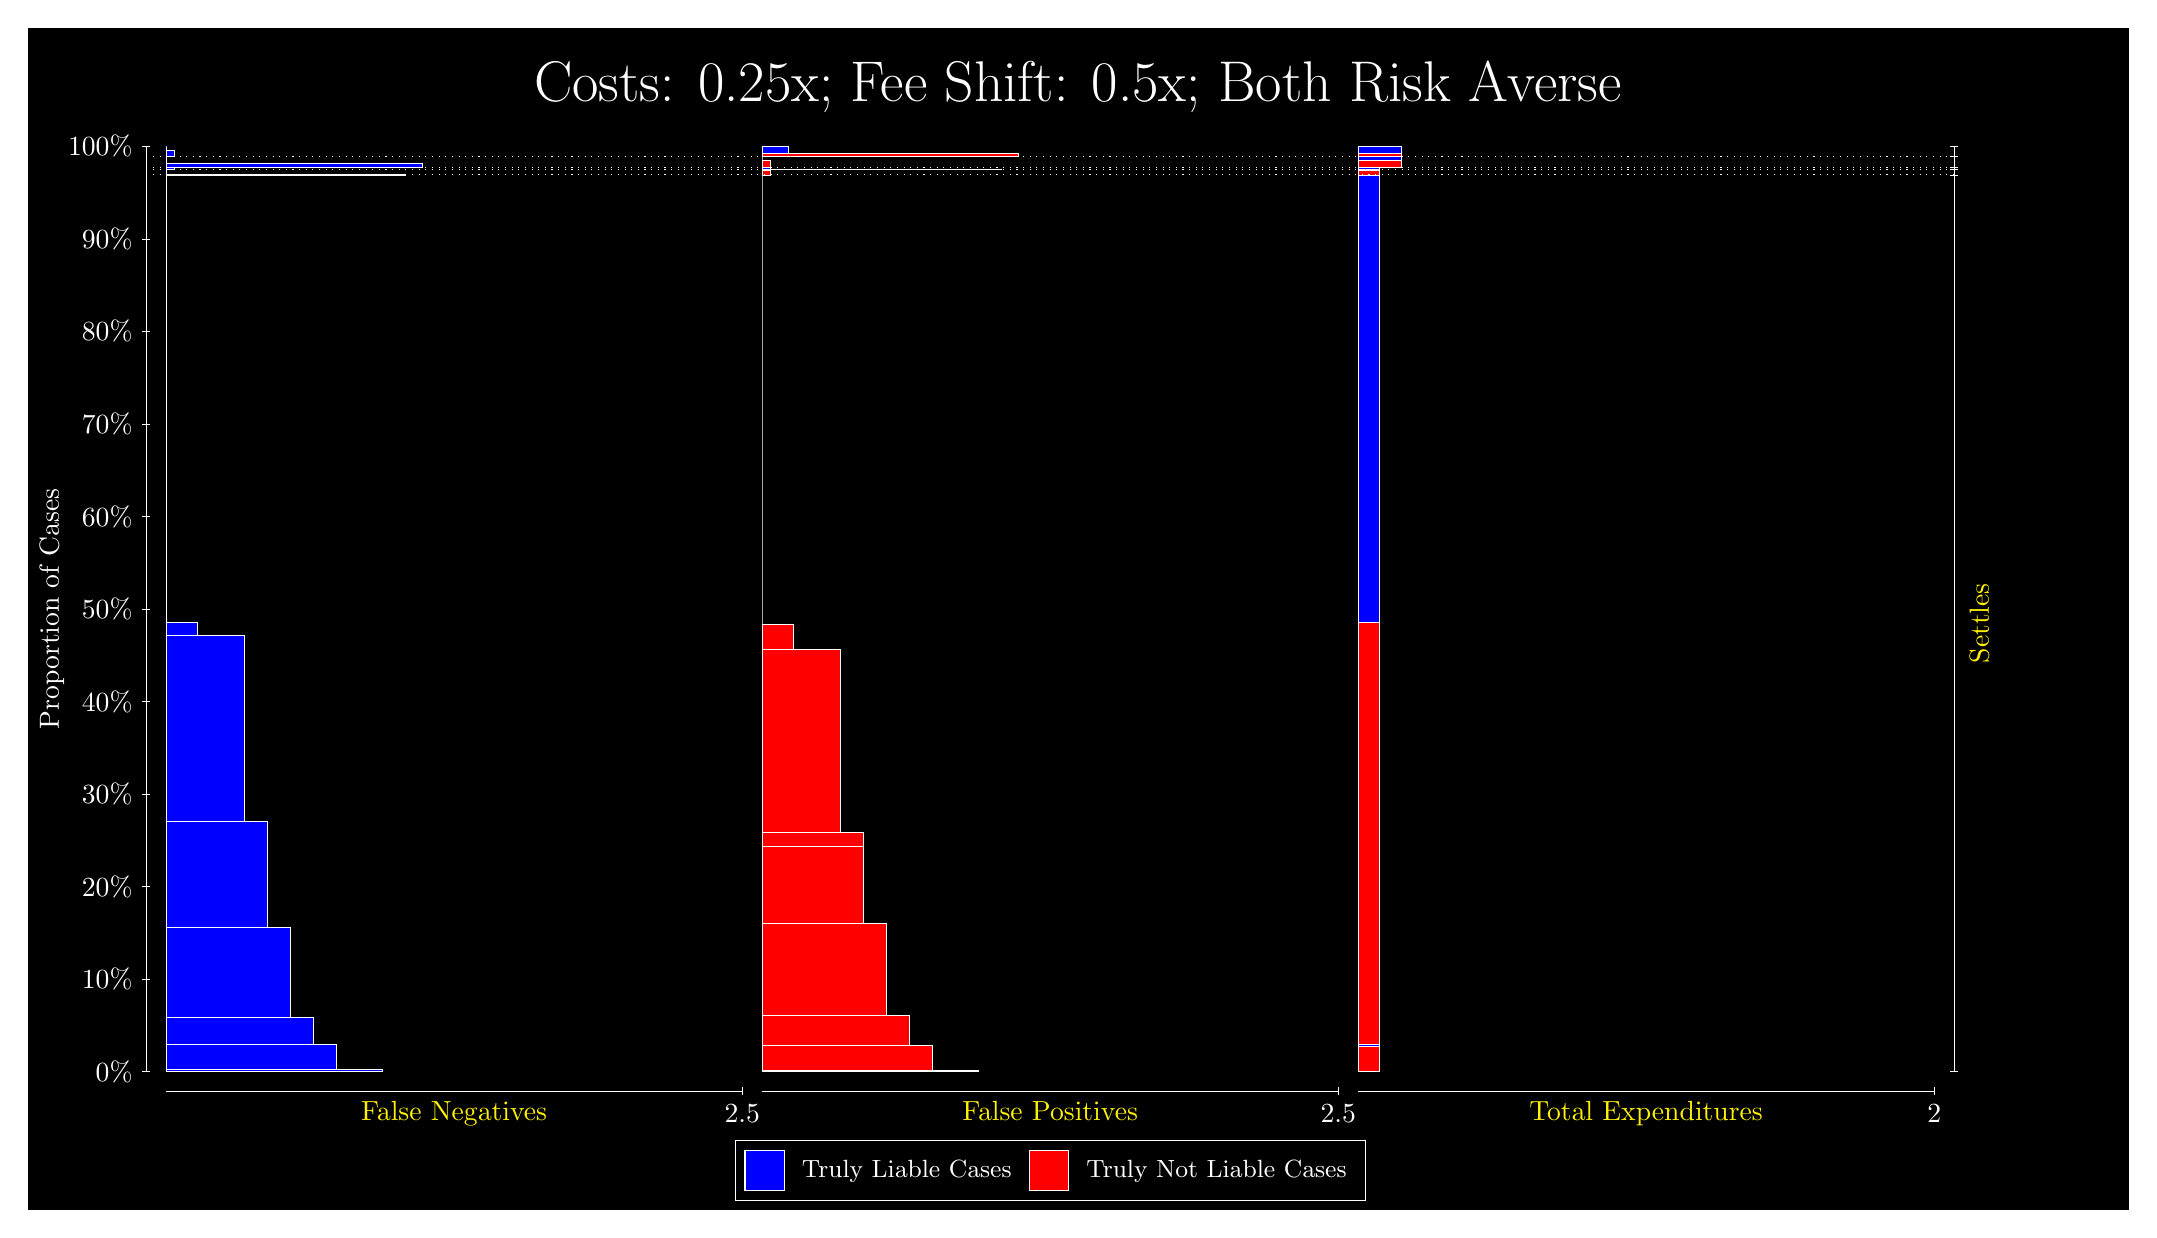
\begin{tikzpicture}
\draw[fill=black] (0,0) rectangle (26.667,15);
\draw[text=white] (0,13.5) rectangle (26.667,15) node[midway] {\huge Costs: 0.25x; Fee Shift: 0.5x; Both Risk Averse};
\draw[white, very thin] (1.5,1.75) -- (1.5,13.5);
\node[rotate=90, text=white, anchor=center] at (0.3, 7.625) {Proportion of Cases};
\draw[white, very thin] (1.45,1.75) -- (1.55,1.75);
\node[text=white, anchor=east] at (1.45, 1.75) {0\%};
\draw[white, very thin] (1.45,2.925) -- (1.55,2.925);
\node[text=white, anchor=east] at (1.45, 2.925) {10\%};
\draw[white, very thin] (1.45,4.1) -- (1.55,4.1);
\node[text=white, anchor=east] at (1.45, 4.1) {20\%};
\draw[white, very thin] (1.45,5.275) -- (1.55,5.275);
\node[text=white, anchor=east] at (1.45, 5.275) {30\%};
\draw[white, very thin] (1.45,6.45) -- (1.55,6.45);
\node[text=white, anchor=east] at (1.45, 6.45) {40\%};
\draw[white, very thin] (1.45,7.625) -- (1.55,7.625);
\node[text=white, anchor=east] at (1.45, 7.625) {50\%};
\draw[white, very thin] (1.45,8.8) -- (1.55,8.8);
\node[text=white, anchor=east] at (1.45, 8.8) {60\%};
\draw[white, very thin] (1.45,9.975) -- (1.55,9.975);
\node[text=white, anchor=east] at (1.45, 9.975) {70\%};
\draw[white, very thin] (1.45,11.15) -- (1.55,11.15);
\node[text=white, anchor=east] at (1.45, 11.15) {80\%};
\draw[white, very thin] (1.45,12.325) -- (1.55,12.325);
\node[text=white, anchor=east] at (1.45, 12.325) {90\%};
\draw[white, very thin] (1.45,13.5) -- (1.55,13.5);
\node[text=white, anchor=east] at (1.45, 13.5) {100\%};

\draw[white, very thin] (24.457,1.75) -- (24.457,13.5);
\draw[white, very thin] (24.407,1.75) -- (24.507,1.75);
\node[anchor=west] at (24.407, 1.75) {};
\draw[white, very thin] (24.407,13.137) -- (24.507,13.137);
\node[anchor=west] at (24.407, 13.137) {};
\draw[white, very thin] (24.407,13.203) -- (24.507,13.203);
\node[anchor=west] at (24.407, 13.203) {};
\draw[white, very thin] (24.407,13.236) -- (24.507,13.236);
\node[anchor=west] at (24.407, 13.236) {};
\draw[white, very thin] (24.407,13.368) -- (24.507,13.368);
\node[anchor=west] at (24.407, 13.368) {};
\draw[white, very thin] (24.407,13.5) -- (24.507,13.5);
\node[anchor=west] at (24.407, 13.5) {};

\draw[white, very thin, fill=blue] (1.75,1.75) rectangle (4.4946,1.7776);
\draw[white, very thin, fill=blue] (1.75,1.7776) rectangle (3.9091,2.0949);
\draw[white, very thin, fill=blue] (1.75,2.0949) rectangle (3.6163,2.4341);
\draw[white, very thin, fill=blue] (1.75,2.4341) rectangle (3.3236,3.5837);
\draw[white, very thin, fill=blue] (1.75,3.5837) rectangle (3.0308,4.9235);
\draw[white, very thin, fill=blue] (1.75,4.9235) rectangle (2.738,7.2927);
\draw[white, very thin, fill=blue] (1.75,7.2927) rectangle (2.1525,7.4544);
\draw[white, very thin, fill=red] (1.75,7.4544) rectangle (1.75,13.137);
\draw[white, very thin, fill=blue] (1.75,13.137) rectangle (4.7873,13.149);
\draw[white, very thin, fill=red] (1.75,13.149) rectangle (1.75,13.203);
\draw[white, very thin, fill=blue] (1.75,13.203) rectangle (1.8598,13.23);
\draw[white, very thin, fill=red] (1.75,13.23) rectangle (1.75,13.236);
\draw[white, very thin, fill=blue] (1.75,13.236) rectangle (5.0069,13.281);
\draw[white, very thin, fill=red] (1.75,13.281) rectangle (1.75,13.368);
\draw[white, very thin, fill=blue] (1.75,13.368) rectangle (1.8598,13.455);
\draw[white, very thin, fill=red] (1.75,13.455) rectangle (1.75,13.5);
\draw[white, very thin, fill=red] (9.3189,1.75) rectangle (12.063,1.7638);
\draw[white, very thin, fill=red] (9.3189,1.7638) rectangle (11.478,2.0786);
\draw[white, very thin, fill=red] (9.3189,2.0786) rectangle (11.185,2.4665);
\draw[white, very thin, fill=red] (9.3189,2.4665) rectangle (10.892,3.6367);
\draw[white, very thin, fill=red] (9.3189,3.6367) rectangle (10.6,4.6165);
\draw[white, very thin, fill=red] (9.3189,4.6165) rectangle (10.6,4.7901);
\draw[white, very thin, fill=red] (9.3189,4.7901) rectangle (10.307,7.1096);
\draw[white, very thin, fill=red] (9.3189,7.1096) rectangle (9.7214,7.433);
\draw[white, very thin, fill=blue] (9.3189,7.433) rectangle (9.3189,13.137);
\draw[white, very thin, fill=red] (9.3189,13.137) rectangle (9.4287,13.192);
\draw[white, very thin, fill=blue] (9.3189,13.192) rectangle (9.3189,13.203);
\draw[white, very thin, fill=red] (9.3189,13.203) rectangle (12.356,13.209);
\draw[white, very thin, fill=blue] (9.3189,13.209) rectangle (9.4287,13.236);
\draw[white, very thin, fill=red] (9.3189,13.236) rectangle (9.4287,13.323);
\draw[white, very thin, fill=blue] (9.3189,13.323) rectangle (9.3189,13.368);
\draw[white, very thin, fill=red] (9.3189,13.368) rectangle (12.576,13.413);
\draw[white, very thin, fill=blue] (9.3189,13.413) rectangle (9.6482,13.5);
\draw[white, very thin, fill=red] (16.888,1.75) rectangle (17.162,2.0733);
\draw[white, very thin, fill=blue] (16.888,2.0733) rectangle (17.162,2.101);
\draw[white, very thin, fill=red] (16.888,2.101) rectangle (17.162,7.4606);
\draw[white, very thin, fill=blue] (16.888,7.4606) rectangle (17.162,13.137);
\draw[white, very thin, fill=red] (16.888,13.137) rectangle (17.162,13.192);
\draw[white, very thin, fill=blue] (16.888,13.192) rectangle (17.162,13.203);
\draw[white, very thin, fill=red] (16.888,13.203) rectangle (17.162,13.209);
\draw[white, very thin, fill=blue] (16.888,13.209) rectangle (17.162,13.236);
\draw[white, very thin, fill=red] (16.888,13.236) rectangle (17.437,13.323);
\draw[white, very thin, fill=blue] (16.888,13.323) rectangle (17.437,13.368);
\draw[white, very thin, fill=red] (16.888,13.368) rectangle (17.437,13.413);
\draw[white, very thin, fill=blue] (16.888,13.413) rectangle (17.437,13.5);
\draw[white, dotted] (1.5,13.137) -- (24.457,13.137);
\draw[white, dotted] (1.5,13.203) -- (24.457,13.203);
\draw[white, dotted] (1.5,13.236) -- (24.457,13.236);
\draw[white, dotted] (1.5,13.368) -- (24.457,13.368);
\draw[white, very thin] (1.75,1.5) -- (9.0689,1.5);
\node[text=yellow, anchor=north] at (5.4094, 1.5) {False Negatives};
\draw[white, very thin] (9.0689,1.45) -- (9.0689,1.55);
\node[text=white, anchor=north] at (9.0689, 1.45) {2.5};

\draw[white, very thin] (9.3189,1.5) -- (16.638,1.5);
\node[text=yellow, anchor=north] at (12.978, 1.5) {False Positives};
\draw[white, very thin] (16.638,1.45) -- (16.638,1.55);
\node[text=white, anchor=north] at (16.638, 1.45) {2.5};

\draw[white, very thin] (16.888,1.5) -- (24.207,1.5);
\node[text=yellow, anchor=north] at (20.547, 1.5) {Total Expenditures};
\draw[white, very thin] (24.207,1.45) -- (24.207,1.55);
\node[text=white, anchor=north] at (24.207, 1.45) {2};

\node[text=yellow, centered, rotate=90] at (24.777, 7.4437) {Settles};





\draw (12.978300999999998,1.5) node[draw=none] (baseCoordinate) {};
\begin{scope}[align=center]
        \matrix[scale=0.5, draw=white, below=0.5cm of baseCoordinate, nodes={draw}, column sep=0.1cm]{
            \node[rectangle, draw, minimum width=0.5cm, minimum height=0.5cm, fill=blue] {}; &
            \node[draw=none, font=\small, text=white] (B) {Truly Liable Cases}; &
            \node[rectangle, draw, minimum width=0.5cm, minimum height=0.5cm, fill=red] {}; &
            \node[draw=none, font=\small, text=white] (B) {Truly Not Liable Cases}; \\
            };
\end{scope}

\end{tikzpicture}
\end{document}